\section{Preliminaries}

\subsection{A discrete grid of robots}

% WORKSPACE 
Let our grid-based workspace be modeled as a graph \ilmath{ G \coloneqq (V, E)}. Let it be a rectangle \ilmath{n_1 \times n_2} where \ilmath{n_1, n_2 \geq 2 \tand n_1, n_2 \in \mathbb{N}}. Label the vertices as \ilmath{V = \set{1, 2, \dots , n_1} \times \set{1, 2, \dots , n_2}}, and denote their \ilmath{x} and \ilmath{y} -coordinates by \ilmath{v_x} and \ilmath{v_y} respectively for any vertex \ilmath{v \in V}. To measure distance, we use the \emph{Manhattan norm} \ilmath{L_1 = \manhattan{v - w} \coloneqq (\abs{v_x - w_x} + \abs{v_y - w_y})}. Using this, the edges can be defined as \ilmath{E = \set{(v, w) \mid \manhattan{v - w} = 1 \text{ for } v, w \in V}}. In other words, nodes are only connected to their up to four immediate neighbors in the plane.

% ROBOTS AND CONFIGURATION
Let there be \ilmath{N \leq (\nngrid)} robots in our workspace. We can identify them by a number \ilmath{r \in R := \set{1, 2, \dots , N} \subset \mathbb{N}}. Let \ilmath{\bot} signify an empty vertex. A \emph{configuration} is then a mapping \ilmath{\conf{} : V \rightarrow \set{1, 2, \dots, N, \bot}} injective upon the robots in \ilmath{R}. Injectivity implies no two vertices in \ilmath{V} can be occupied at once, so there will always be exactly \ilmath{(\nngrid - N)} empty squares in the grid.

% CONFIGURATION INVERSE
The \emph{inverse} of a configuration \ilmath{\iconf{}{r} = (x, y), \; r \in R} is the \emph{position} of a robot. The robots move synchronously and in parallel, up to a single edge at a time. A valid (no-collision) configuration \ilmath{\conf{1}} can thus be \emph{transformed} into another valid configuration \ilmath{\conf{2}} in a \emph{single step} if and only if:

% TRANSFORMATION REQUIREMENTS
\begin{align}
	& \parens{\iconf{1}{r} = \iconf{2}{r} \lor (\iconf{1}{r}, \iconf{2}{r}) \in E, \; \forall r \in R}\label{req:limited_movement}\\
	\land & \parens{\nconf{1}{v} = \nconf{2}{w} \Rightarrow \nconf{2}{v} \neq \nconf{1}{w}, \; \forall v, w \in V}\label{req:no_swaps}
\end{align}

In other words, \cref{req:limited_movement} implies a robot can stay in place or move to a neighboring square at every step, while \cref{req:no_swaps} forbids two robots from swapping places in a single transformation step (and they can never occupy the same vertex), equivalent to a collision in the real world.

% SCHEDULE
Denote a single transformation step as \ilmath{\conf{1} \rightarrow \conf{2}}. A \emph{schedule} is a sequence of transformation steps \ilmath{\conf{1} \rightarrow \conf{2} \rightarrow \cdots \rightarrow \conf{k}}. A configuration \ilmath{\conf{s}} can be transformed into a configuration \ilmath{\conf{t}} if there exists a schedule \ilmath{\conf{s} \rightarrow \conf{s + 1} \rightarrow \cdots \rightarrow \conf{t - 1} \rightarrow \conf{t}}.


% PROBLEM DEFINITION
\begin{definition}\label{def:motion_planning_problem}
	Given a start configuration \ilmath{\conf{s}} and a target configuration \ilmath{\conf{t}} of a workspace, the \emph{motion planning problem} ask to find a \emph{schedule} that transforms \ilmath{\conf{s}} into \ilmath{\conf{t}}.
\end{definition}

\begin{remark}\label{remark:reachability}
	For a \ilmath{2 \times 2} square and any \ilmath{1 \times n} rectangle, where \ilmath{n \geq 2}, there exist pairs of configurations that are not reachable from each other via any schedule. See \cref{fig:reachability} for an example. For any other rectangular workspace there always exists such a schedule. 
\end{remark}
% IMPOSSIBLE 2*2 SQUARE FIGURE
\begin{figure}[h]
	\centering
	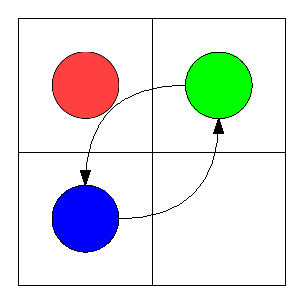
\includegraphics[width=4cm]{include/impossible_2x2.eps}
	\caption{A minimal example of an unsolvable motion planning problem: there exists no valid schedule which swaps the green and blue robots.}\label{fig:reachability}
\end{figure}

% MAKESPAN
\begin{definition}\label{def:makespan}
	The number of single transformation steps in a schedule is called the \emph{makespan} of that schedule.
\end{definition}

\begin{definition}\label{def:optimality}
Let \ilmath{\Sigma_{s \rightarrow t}} denote the set of all valid schedules for some pair of configurations \ilmath{\conf{s}} and \ilmath{\conf{t}}.
	A schedule \ilmath{S_\text{opt}} is \emph{optimal} with respect to some cost function \ilmath{f : S \rightarrow \mathbb{N}} mapping all valid schedules \ilmath{S} to some integer value if and only if \ilmath{f(S) \geq f(\sopt)} for all such valid schedules \ilmath{S}.
\end{definition}

% M3PP -- MINIMUM MAKESPAN MOTION PLANNING PROBLEM
\begin{definition}\label{def:m3pp}
	Let the makespan of a schedule be such a cost function: \ilmath{M : S \rightarrow} (\textit{number of tranformation steps in S}). The \emph{minimum makespan motion planning problem} asks to find an \emph{optimal} schedule with respect to the makespan \ilmath{M} for some input start and target configuration.
\end{definition}

\begin{remark}
	The \emph{minimum makespan} for any motion planning problem with inputs \ilmath{\conf{s}} and \ilmath{\conf{t}} is bounded below by \ilmath{\max(\set{\manhattan{\iconf{s}{r}, \; \iconf{t}{r}}, \; r \in R})}.
\end{remark}

\begin{definition}
	Let the aforementioned lower bound to a schedule with makespan \ilmath{M} be denoted by \ilmath{L}. The \ilmath{\emph{stretch factor}} for that schedule is then defined as \ilmath{\frac{M}{L} \geq 1}.
\end{definition}

Let the cost of an optimal schedule \ilmath{\sopt} to some motion planning problem with respect to some cost function \ilmath{f : S \rightarrow \mathbb{N}} be denoted by \ilmath{f(\sopt)}. A \ilmath{\rho}\emph{-approximation algorithm} is defined as an algorithm that always gives a schedule with cost within a \ilmath{\rho} factor of the optimal solution:
\begin{align}\label{def:approximation_algorithm}
	f(\sopt) \leq f(S_\text{approx.}) \leq \rho f(\sopt), \; \rho > 1
\end{align}

\begin{remark}
	Stretch implies approximation \dots
\end{remark}



\note{How to get robot colorings in here?}

\subsection{Some notation}

\begin{definition}
	\ilmath{O(g(x))}
\end{definition}



